\documentclass{standalone}
\usepackage{tikz}
\usetikzlibrary{patterns, positioning}


\begin{document}
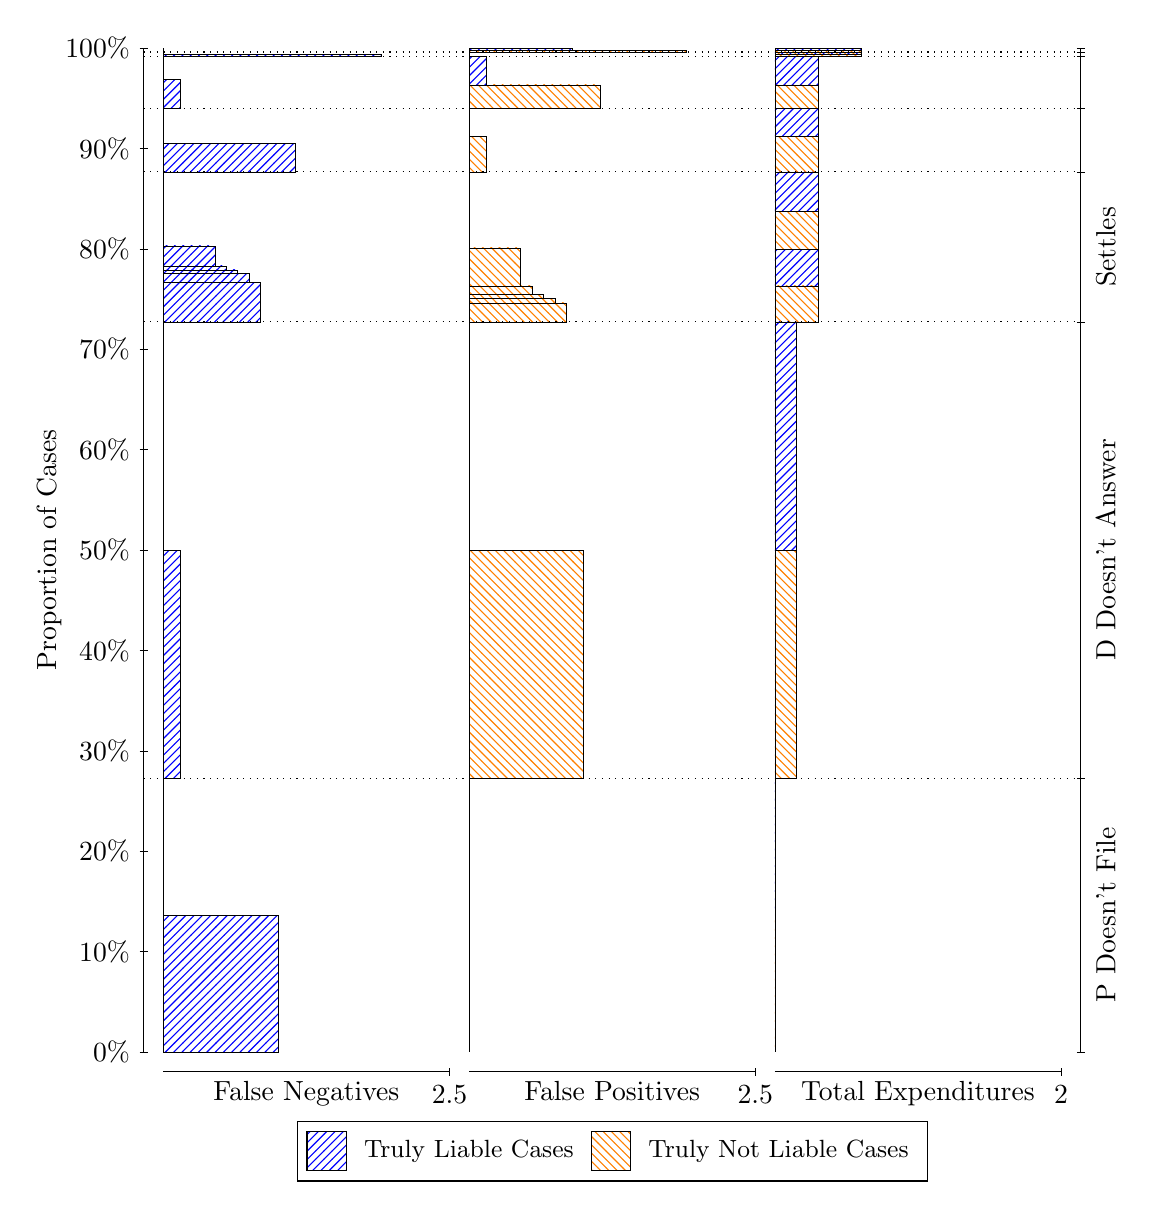
\begin{tikzpicture}
\draw[black, very thin] (1.5,1.75) -- (1.5,14.5);
\node[rotate=90, text=black, anchor=center] at (0.3, 8.125) {Proportion of Cases};
\draw[black, very thin] (1.45,1.75) -- (1.55,1.75);
\node[text=black, anchor=east] at (1.45, 1.75) {0\%};
\draw[black, very thin] (1.45,3.025) -- (1.55,3.025);
\node[text=black, anchor=east] at (1.45, 3.025) {10\%};
\draw[black, very thin] (1.45,4.3) -- (1.55,4.3);
\node[text=black, anchor=east] at (1.45, 4.3) {20\%};
\draw[black, very thin] (1.45,5.575) -- (1.55,5.575);
\node[text=black, anchor=east] at (1.45, 5.575) {30\%};
\draw[black, very thin] (1.45,6.85) -- (1.55,6.85);
\node[text=black, anchor=east] at (1.45, 6.85) {40\%};
\draw[black, very thin] (1.45,8.125) -- (1.55,8.125);
\node[text=black, anchor=east] at (1.45, 8.125) {50\%};
\draw[black, very thin] (1.45,9.4) -- (1.55,9.4);
\node[text=black, anchor=east] at (1.45, 9.4) {60\%};
\draw[black, very thin] (1.45,10.675) -- (1.55,10.675);
\node[text=black, anchor=east] at (1.45, 10.675) {70\%};
\draw[black, very thin] (1.45,11.95) -- (1.55,11.95);
\node[text=black, anchor=east] at (1.45, 11.95) {80\%};
\draw[black, very thin] (1.45,13.225) -- (1.55,13.225);
\node[text=black, anchor=east] at (1.45, 13.225) {90\%};
\draw[black, very thin] (1.45,14.5) -- (1.55,14.5);
\node[text=black, anchor=east] at (1.45, 14.5) {100\%};

\draw[black, very thin] (13.4,1.75) -- (13.4,14.5);
\draw[black, very thin] (13.35,1.75) -- (13.45,1.75);
\node[anchor=west] at (13.35, 1.75) {};
\draw[black, very thin] (13.35,5.2273) -- (13.45,5.2273);
\node[anchor=west] at (13.35, 5.2273) {};
\draw[black, very thin] (13.35,11.023) -- (13.45,11.023);
\node[anchor=west] at (13.35, 11.023) {};
\draw[black, very thin] (13.35,12.928) -- (13.45,12.928);
\node[anchor=west] at (13.35, 12.928) {};
\draw[black, very thin] (13.35,13.733) -- (13.45,13.733);
\node[anchor=west] at (13.35, 13.733) {};
\draw[black, very thin] (13.35,14.398) -- (13.45,14.398);
\node[anchor=west] at (13.35, 14.398) {};
\draw[black, very thin] (13.35,14.449) -- (13.45,14.449);
\node[anchor=west] at (13.35, 14.449) {};
\draw[black, very thin] (13.35,14.5) -- (13.45,14.5);
\node[anchor=west] at (13.35, 14.5) {};

\draw[black, very thin, pattern color=blue, pattern=north east lines] (1.75,1.75) rectangle (3.2033,3.4886);
\draw[black, very thin, pattern color=orange, pattern=north west lines] (1.75,3.4886) rectangle (1.75,5.2273);
\draw[black, very thin, pattern color=blue, pattern=north east lines] (1.75,5.2273) rectangle (1.968,8.125);
\draw[black, very thin, pattern color=orange, pattern=north west lines] (1.75,8.125) rectangle (1.75,11.023);
\draw[black, very thin, pattern color=blue, pattern=north east lines] (1.75,11.023) rectangle (2.9853,11.527);
\draw[black, very thin, pattern color=blue, pattern=north east lines] (1.75,11.527) rectangle (2.84,11.64);
\draw[black, very thin, pattern color=blue, pattern=north east lines] (1.75,11.64) rectangle (2.6947,11.682);
\draw[black, very thin, pattern color=blue, pattern=north east lines] (1.75,11.682) rectangle (2.5493,11.733);
\draw[black, very thin, pattern color=blue, pattern=north east lines] (1.75,11.733) rectangle (2.404,11.987);
\draw[black, very thin, pattern color=orange, pattern=north west lines] (1.75,11.987) rectangle (1.75,12.928);
\draw[black, very thin, pattern color=blue, pattern=north east lines] (1.75,12.928) rectangle (3.4213,13.285);
\draw[black, very thin, pattern color=orange, pattern=north west lines] (1.75,13.285) rectangle (1.75,13.733);
\draw[black, very thin, pattern color=blue, pattern=north east lines] (1.75,13.733) rectangle (1.968,14.099);
\draw[black, very thin, pattern color=orange, pattern=north west lines] (1.75,14.099) rectangle (1.75,14.398);
\draw[black, very thin, pattern color=blue, pattern=north east lines] (1.75,14.398) rectangle (4.5113,14.421);
\draw[black, very thin, pattern color=orange, pattern=north west lines] (1.75,14.421) rectangle (1.75,14.449);
\draw[black, very thin, pattern color=orange, pattern=north west lines] (1.75,14.449) rectangle (1.75,14.472);
\draw[black, very thin, pattern color=blue, pattern=north east lines] (1.75,14.472) rectangle (1.75,14.5);
\draw[black, very thin, pattern color=orange, pattern=north west lines] (5.6333,1.75) rectangle (5.6333,3.4886);
\draw[black, very thin, pattern color=blue, pattern=north east lines] (5.6333,3.4886) rectangle (5.6333,5.2273);
\draw[black, very thin, pattern color=orange, pattern=north west lines] (5.6333,5.2273) rectangle (7.0867,8.125);
\draw[black, very thin, pattern color=blue, pattern=north east lines] (5.6333,8.125) rectangle (5.6333,11.023);
\draw[black, very thin, pattern color=orange, pattern=north west lines] (5.6333,11.023) rectangle (6.8687,11.262);
\draw[black, very thin, pattern color=orange, pattern=north west lines] (5.6333,11.262) rectangle (6.7233,11.322);
\draw[black, very thin, pattern color=orange, pattern=north west lines] (5.6333,11.322) rectangle (6.578,11.371);
\draw[black, very thin, pattern color=orange, pattern=north west lines] (5.6333,11.371) rectangle (6.4327,11.48);
\draw[black, very thin, pattern color=orange, pattern=north west lines] (5.6333,11.48) rectangle (6.2873,11.963);
\draw[black, very thin, pattern color=blue, pattern=north east lines] (5.6333,11.963) rectangle (5.6333,12.928);
\draw[black, very thin, pattern color=orange, pattern=north west lines] (5.6333,12.928) rectangle (5.8513,13.376);
\draw[black, very thin, pattern color=blue, pattern=north east lines] (5.6333,13.376) rectangle (5.6333,13.733);
\draw[black, very thin, pattern color=orange, pattern=north west lines] (5.6333,13.733) rectangle (7.3047,14.032);
\draw[black, very thin, pattern color=blue, pattern=north east lines] (5.6333,14.032) rectangle (5.8513,14.398);
\draw[black, very thin, pattern color=orange, pattern=north west lines] (5.6333,14.398) rectangle (5.6333,14.425);
\draw[black, very thin, pattern color=blue, pattern=north east lines] (5.6333,14.425) rectangle (5.6333,14.449);
\draw[black, very thin, pattern color=orange, pattern=north west lines] (5.6333,14.449) rectangle (8.3947,14.472);
\draw[black, very thin, pattern color=blue, pattern=north east lines] (5.6333,14.472) rectangle (6.9413,14.5);
\draw[black, very thin, pattern color=orange, pattern=north west lines] (9.5167,1.75) rectangle (9.5167,3.4886);
\draw[black, very thin, pattern color=blue, pattern=north east lines] (9.5167,3.4886) rectangle (9.5167,5.2273);
\draw[black, very thin, pattern color=orange, pattern=north west lines] (9.5167,5.2273) rectangle (9.7892,8.125);
\draw[black, very thin, pattern color=blue, pattern=north east lines] (9.5167,8.125) rectangle (9.7892,11.023);
\draw[black, very thin, pattern color=orange, pattern=north west lines] (9.5167,11.023) rectangle (10.062,11.48);
\draw[black, very thin, pattern color=blue, pattern=north east lines] (9.5167,11.48) rectangle (10.062,11.941);
\draw[black, very thin, pattern color=orange, pattern=north west lines] (9.5167,11.941) rectangle (10.062,12.424);
\draw[black, very thin, pattern color=blue, pattern=north east lines] (9.5167,12.424) rectangle (10.062,12.928);
\draw[black, very thin, pattern color=orange, pattern=north west lines] (9.5167,12.928) rectangle (10.062,13.376);
\draw[black, very thin, pattern color=blue, pattern=north east lines] (9.5167,13.376) rectangle (10.062,13.733);
\draw[black, very thin, pattern color=orange, pattern=north west lines] (9.5167,13.733) rectangle (10.062,14.032);
\draw[black, very thin, pattern color=blue, pattern=north east lines] (9.5167,14.032) rectangle (10.062,14.398);
\draw[black, very thin, pattern color=orange, pattern=north west lines] (9.5167,14.398) rectangle (10.607,14.425);
\draw[black, very thin, pattern color=blue, pattern=north east lines] (9.5167,14.425) rectangle (10.607,14.449);
\draw[black, very thin, pattern color=orange, pattern=north west lines] (9.5167,14.449) rectangle (10.607,14.472);
\draw[black, very thin, pattern color=blue, pattern=north east lines] (9.5167,14.472) rectangle (10.607,14.5);
\draw[black, dotted] (1.5,5.2273) -- (13.4,5.2273);
\draw[black, dotted] (1.5,11.023) -- (13.4,11.023);
\draw[black, dotted] (1.5,12.928) -- (13.4,12.928);
\draw[black, dotted] (1.5,13.733) -- (13.4,13.733);
\draw[black, dotted] (1.5,14.398) -- (13.4,14.398);
\draw[black, dotted] (1.5,14.449) -- (13.4,14.449);
\draw[black, very thin] (1.75,1.5) -- (5.3833,1.5);
\node[text=black, anchor=north] at (3.5667, 1.5) {False Negatives};
\draw[black, very thin] (5.3833,1.45) -- (5.3833,1.55);
\node[text=black, anchor=north] at (5.3833, 1.45) {2.5};

\draw[black, very thin] (5.6333,1.5) -- (9.2667,1.5);
\node[text=black, anchor=north] at (7.45, 1.5) {False Positives};
\draw[black, very thin] (9.2667,1.45) -- (9.2667,1.55);
\node[text=black, anchor=north] at (9.2667, 1.45) {2.5};

\draw[black, very thin] (9.5167,1.5) -- (13.15,1.5);
\node[text=black, anchor=north] at (11.333, 1.5) {Total Expenditures};
\draw[black, very thin] (13.15,1.45) -- (13.15,1.55);
\node[text=black, anchor=north] at (13.15, 1.45) {2};

\node[text=black, centered, rotate=90] at (13.72, 3.4886) {P Doesn't File};
\node[text=black, centered, rotate=90] at (13.72, 8.125) {D Doesn't Answer};
\node[text=black, centered, rotate=90] at (13.72, 11.975) {Settles};





\draw (7.449999999999999,1.5) node[draw=none] (baseCoordinate) {};
\begin{scope}[align=center]
        \matrix[scale=0.5, draw=black, below=0.5cm of baseCoordinate, nodes={draw}, column sep=0.1cm]{
            \node[rectangle, draw, minimum width=0.5cm, minimum height=0.5cm, pattern color=blue, pattern=north east lines] {}; &
            \node[draw=none, font=\small, text=black] (B) {Truly Liable Cases}; &
            \node[rectangle, draw, minimum width=0.5cm, minimum height=0.5cm, pattern color=orange, pattern=north west lines] {}; &
            \node[draw=none, font=\small, text=black] (B) {Truly Not Liable Cases}; \\
            };
\end{scope}

\end{tikzpicture}
\end{document}